% 编译指令:
% xelatex -8bit -synctex=1 -interaction=nonstopmode -shell-escape %.tex | txs:///view-pdf-internal -

\documentclass{article}
\usepackage{listings}
\usepackage{xcolor}
\usepackage[english]{babel}
\usepackage{amsmath,amsthm}
\usepackage{amsfonts}
\usepackage[longend,ruled,linesnumbered]{algorithm2e}
\usepackage{fancyhdr}
\usepackage{ctex}
\usepackage{array}
\usepackage{listings}
\usepackage{color}
\usepackage{graphicx}
\usepackage{geometry}
\usepackage{minted}
\usepackage{float}

% 定义Julia语言样式
\lstdefinelanguage{Julia}%
{morekeywords={abstract,break,case,catch,const,continue,do,else,elseif,%
		end,export,false,for,function,immutable,import,importall,if,in,%
		macro,module,otherwise,quote,return,switch,true,try,type,typealias,%
		using,while},%
	sensitive=true,%
	alsoother={$},%
	morecomment=[l]\#,%
	morecomment=[n]{\#=}{=\#},%
	morestring=[s]{"}{"},%
	morestring=[m]{'}{'},%
}[keywords,comments,strings]

% 设置代码样式
\lstset{
	language=Julia, % 设置语言为Julia
	basicstyle=\ttfamily, % 设置基本样式为等宽字体
	keywordstyle=\bfseries\color{blue}, % 设置关键字样式为蓝色粗体
	commentstyle=\itshape\color{gray}, % 设置注释样式为灰色斜体
	showstringspaces=false, % 不显示代码中的空格
	numbers=left, % 行号显示在左侧
	numberstyle=\tiny\color{gray}, % 行号样式为小号灰色
	breaklines=true, % 自动换行
	frame=single, % 为代码添加边框
	backgroundcolor=\color{lightgray!10}, % 设置背景色为浅灰色
	captionpos=b % 设置标题位置为底部
}

\begin{document}
	\section*{spectrogram}
	
	\begin{minted}{julia}
		s, = spectrogram(x)
	\end{minted}
	
	返回输入信号 x 的短时傅立叶变换(STFT)。s 的每列包含 x 的短期、时间局部化频率内容的估计。s 的幅度平方被称为 x[1] 的频谱图时间-频率表示。

	\begin{minted}{julia}
		s, = spectrogram(x, window)
	\end{minted}
	
	使用 window 将信号划分为段并执行开窗。
	
	\begin{minted}{julia}
		s, = spectrogram(x, window, noverlap)
	\end{minted}
	
	使用相邻线段之间重叠的 noverlap 样本。
	
	\begin{minted}{julia}
		s, = spectrogram(x, window, noverlap, nfft)
	\end{minted}
	
	使用 nfft 采样点计算离散傅立叶变换。

	\begin{minted}{julia}
		s, w, t = spectrogram(___)
	\end{minted}
	
	返回归一化频率向量 w 和计算 STFT 的时间时刻向量 t。该语法可以包含前面语法中输入参数的任意组合。
	
	\begin{minted}{julia}
		s, f, t = spectrogram(___, fs)
	\end{minted}
	
	返回循环频率的矢量 f,用采样率 fs 表示。fs 必须是声谱图的第五个输入。要输入采样率并仍然使用前面可选参数的默认值,请将这些参数指定为空,[]。
	
	\begin{minted}{julia}
		s, w, t = spectrogram(x, window, noverlap, w)
	\end{minted}
	
	以 w.w 中指定的归一化频率返回 STFT。w 必须至少有两个元素,否则函数会将其解释为 nfft。
	
	\begin{minted}{julia}
		s, f, t = spectrogram(x, window, noverlap, f, fs)
	\end{minted}
	
	以 f 中指定的循环频率返回 STFT。f 必须至少有两个元素,否则函数会将其解释为 nfft。
	
	\begin{minted}{julia}
		_, _, _, ps = spectrogram(___)
	\end{minted}
	
	还会返回一个与 x 的频谱图成正比的矩阵 ps。
	
	\begin{itemize}
		\item 如果指定频谱类型为 "psd",则 ps 的每一列都包含一个窗口分段的功率谱密度(PSD)估计值。
		
		\item 如果指定频谱类型为 "power",则 ps 的每一列都包含一个窗口分段的功率谱估计值。
	\end{itemize}	
	
	
	\begin{minted}{julia}
		_ = spectrogram(___, "reassigned")
	\end{minted}
	
	将每个 PSD 或功率谱估算值重新分配到其能量中心的位置。如果您的信号包含定位良好的时间或频谱成分,那么该选项生成的频谱图会更清晰。
	
	\begin{minted}{julia}
		_, _, _, ps, fc, tc = spectrogram(___)
	\end{minted}
	
	还会返回两个矩阵 fc 和 tc,其中包含每个 PSD 或功率谱估计值的能量中心频率和时间。
	
	\begin{minted}{julia}
		___ = spectrogram(___, freqrange)
	\end{minted}
	
	返回 freqrange 指定频率范围内的 PSD 或功率谱估计值。freqrange 的有效选项为 "onesided"、"twosided" 和 "centered"。

	\begin{minted}{julia}
		___ = spectrogram(___, Name,Value)
	\end{minted}
	
	使用名称值参数指定其他选项。选项包括最小阈值和输出时间维度。
	
	\begin{minted}{julia}
		___ = spectrogram(___, spectrumtype)
	\end{minted}

	如果频谱类型指定为 "psd",则返回短期交叉功率谱密度估计值;如果频谱类型指定为 "power",则返回短期交叉功率谱估计值。

	\begin{minted}[showspaces=false]{julia}
		spectrogram(___) 
	\end{minted}

	在没有输出参数的情况下,在当前图形窗口中绘制交叉谱图。

	\begin{minted}[showspaces=false]{julia}
		spectrogram(___, freqloc) 
	\end{minted}

	指定绘制频率的轴。将 freqloc 指定为 "xaxis" 或 "yaxis"。

	\lstinputlisting[caption={频谱图的默认值}, label={julia1}]{hw5(1).jl}
	\begin{figure}[H]
		\centering
		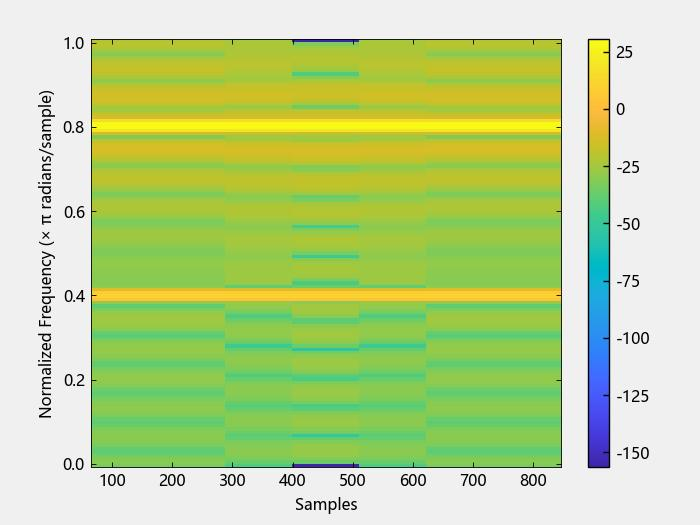
\includegraphics{hw5(1).jpeg}
		\caption{Listing1结果图}
		\label{fig1}
	\end{figure}
	\lstinputlisting[caption={沿x轴的频率}, label={julia2}]{hw5(2).jl}
	\begin{figure}[htbp]
		\centering
		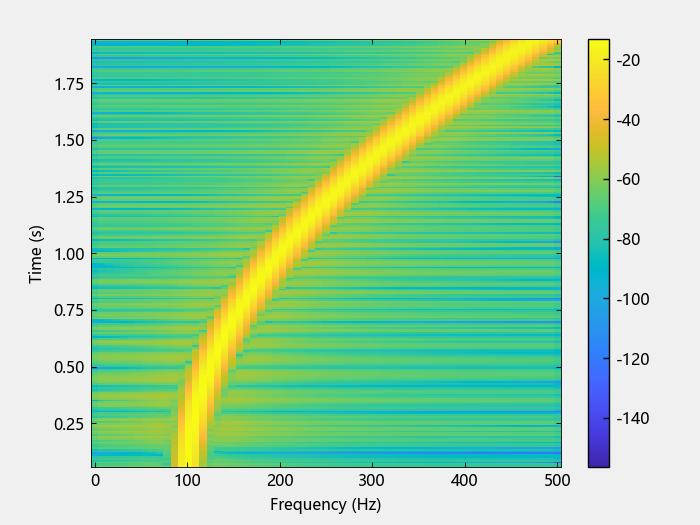
\includegraphics{hw5(2)-1.jpeg}
	%	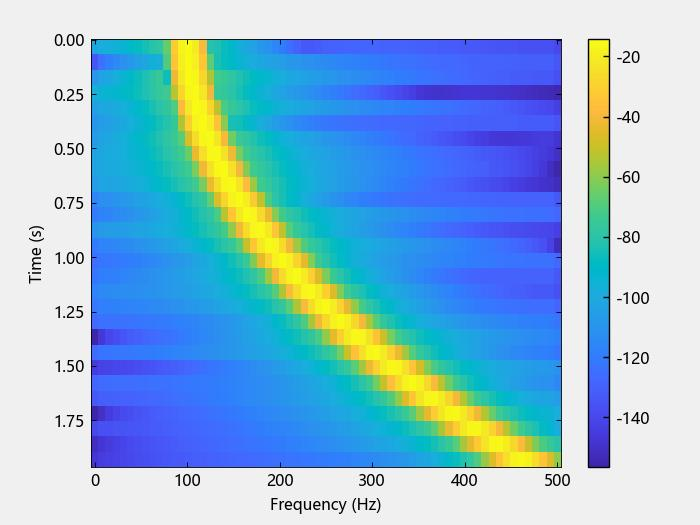
\includegraphics{hw5(2)-2.jpeg}
		\caption{Listing2结果图1}
		\label{fig2-1}
	\end{figure}
	\begin{figure}[htbp]
		\centering
		%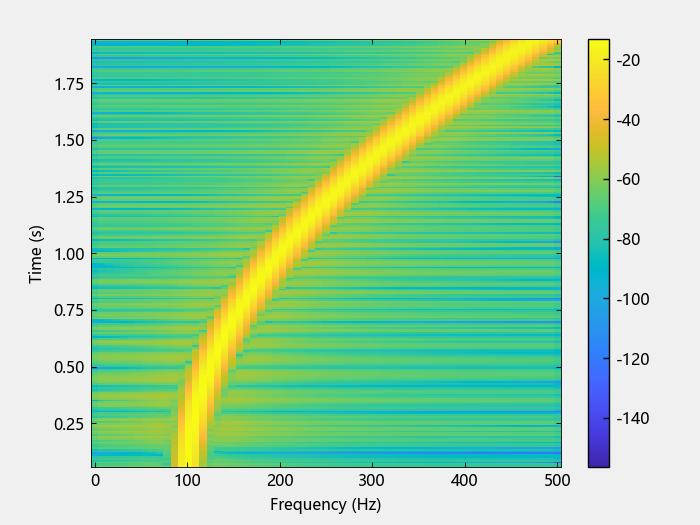
\includegraphics{hw5(2)-1.jpeg}
		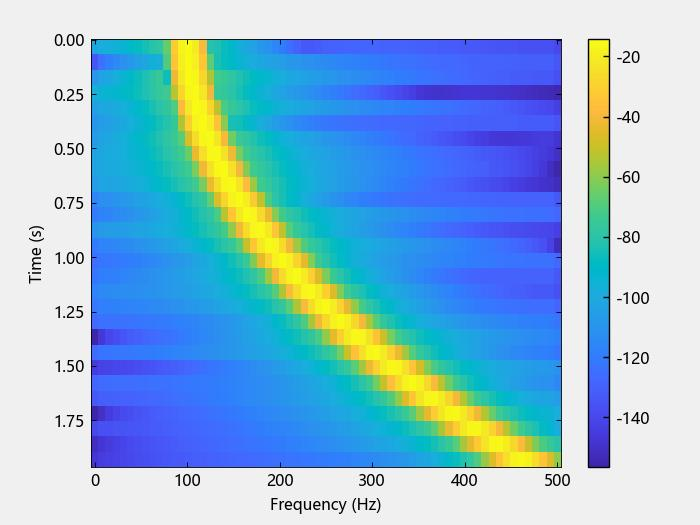
\includegraphics{hw5(2)-2.jpeg}
		\caption{Listing2结果图2}
		\label{fig2-2}
	\end{figure}
	\lstinputlisting[caption={线性调频的功率谱密度}, label={julia3}]{hw5(3).jl}
	\begin{figure}[htbp]
		\centering
		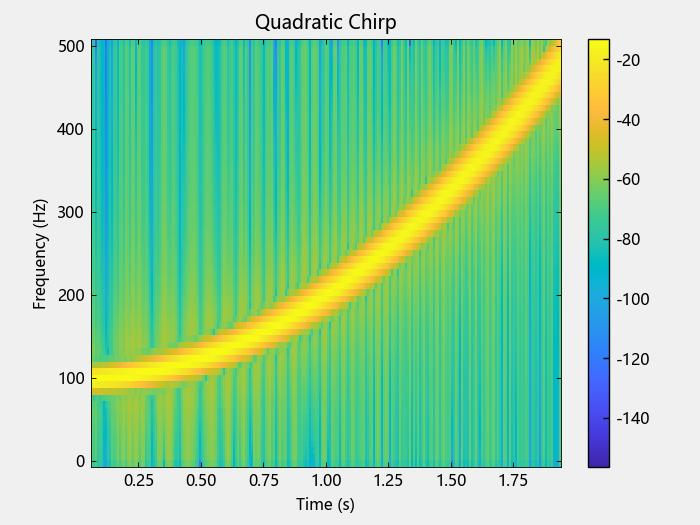
\includegraphics{hw5(3)-1.jpeg}
		\caption{Listing3结果图1}
		\label{fig3-1}
	\end{figure}
		\begin{figure}[htbp]
		\centering
		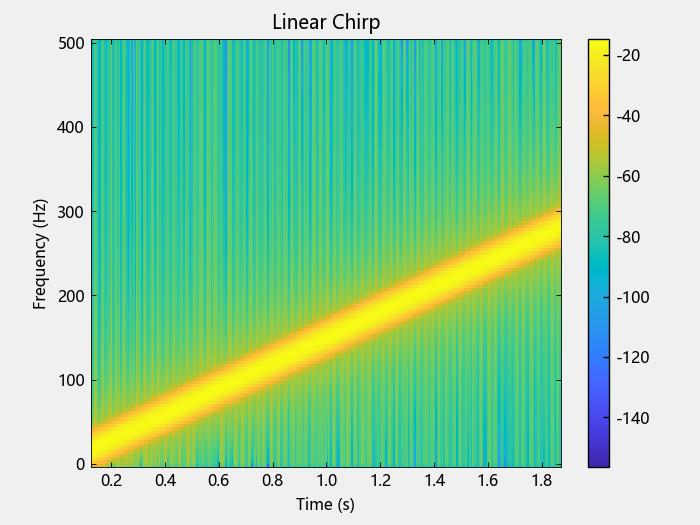
\includegraphics{hw5(3)-2.jpeg}
		\caption{Listing3结果图2}
		\label{fig3-2}
	\end{figure}
		\begin{figure}[htbp]
		\centering
		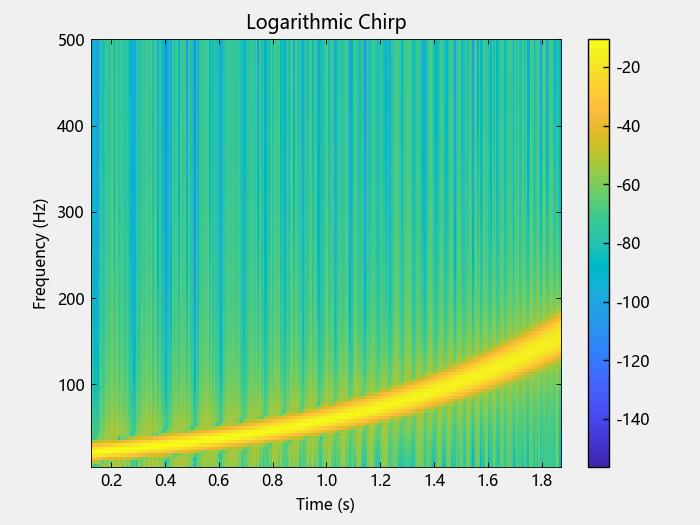
\includegraphics{hw5(3)-3.jpeg}
		\caption{Listing3结果图3}
		\label{fig3-3}
	\end{figure}
	
	\lstinputlisting[caption={频谱图和瞬时频率}, label={julia4}]{hw5(4).jl}
	\begin{figure}[htbp]
		\centering
		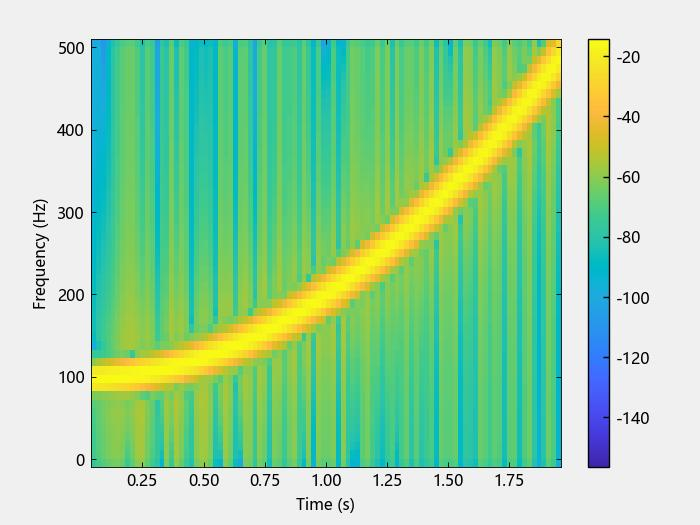
\includegraphics{hw5(4).jpeg}
		\caption{Listing4结果图}
		\label{fig4}
	\end{figure}
	\lstinputlisting[caption={复信号频谱图}, label={julia5}]{hw5(5).jl}
	\begin{figure}[htbp]
		\centering
		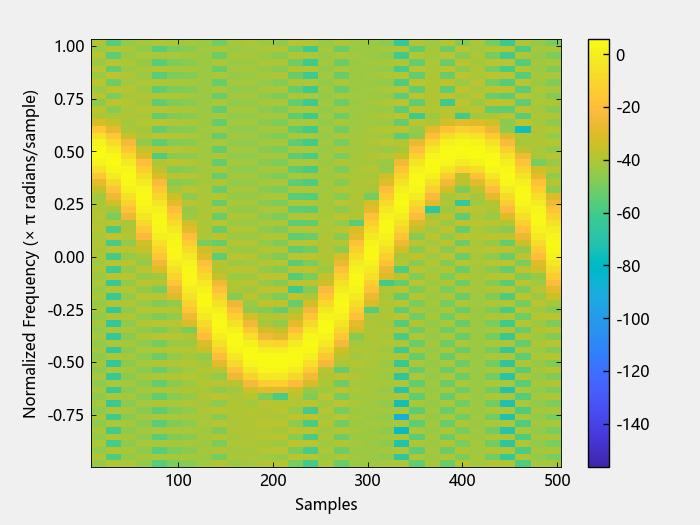
\includegraphics{hw5(5).jpeg}
		\caption{Listing5结果图}
		\label{fig5}
	\end{figure}
	\lstinputlisting[caption={二次线性调频的重新分配频谱图}, label={julia6}]{hw5(6).jl}
	\begin{figure}[htbp]
		\centering
		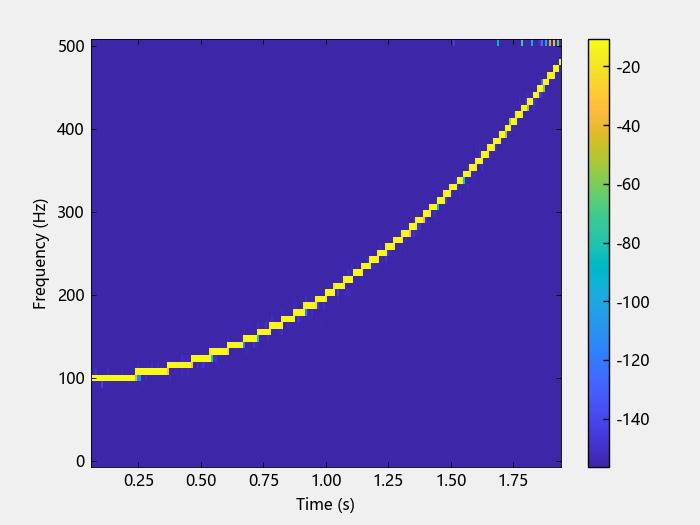
\includegraphics{hw5(6).jpeg}
		\caption{Listing6结果图}
		\label{fig6}
	\end{figure}
	\lstinputlisting[caption={带阈值的频谱图}, label={julia7}]{hw5(7).jl}
	\begin{figure}[htbp]
		\centering
		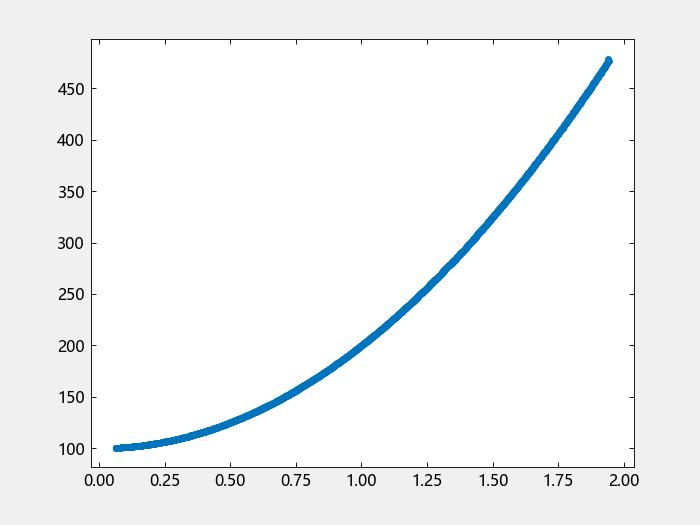
\includegraphics{hw5(7).jpeg}
		\caption{Listing7结果图}
		\label{fig7}
	\end{figure}
	\lstinputlisting[caption={频谱图重新分配和阈值处理}, label={julia8}]{hw5(8).jl}
	\begin{figure}[htbp]
		\centering
		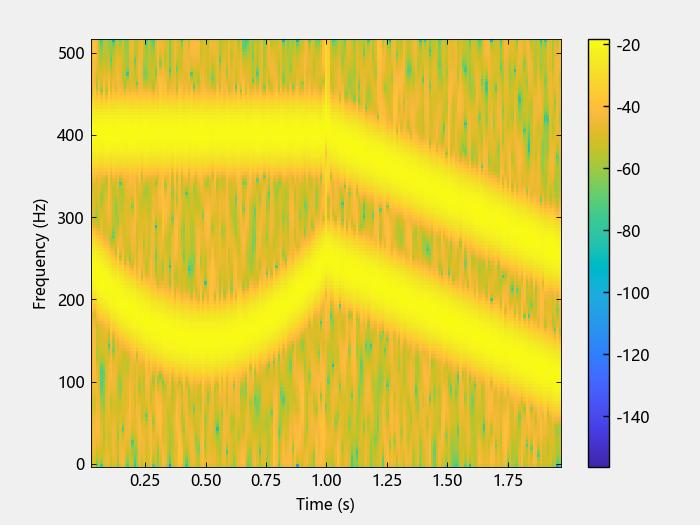
\includegraphics{hw5(8)-1.jpeg}
		\caption{Listing8结果图1}
		\label{fig8-1}
	\end{figure}
	\begin{figure}[htbp]
		\centering
		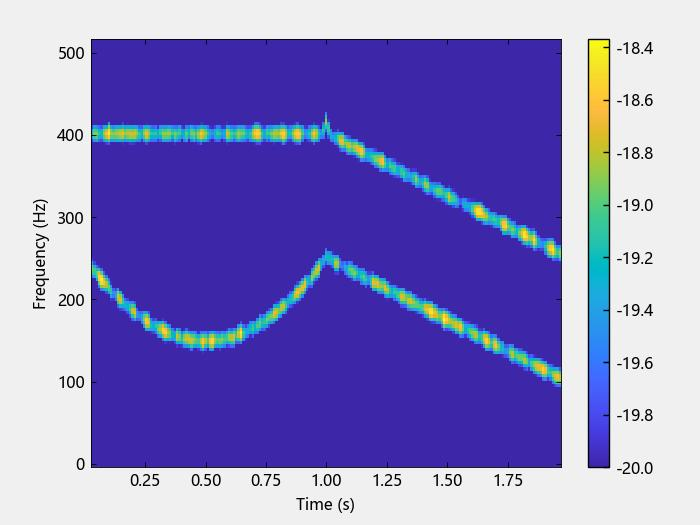
\includegraphics{hw5(8)-2.jpeg}
		\caption{Listing8结果图2}
		\label{fig8-2}
	\end{figure}
	\begin{figure}[htbp]
		\centering
		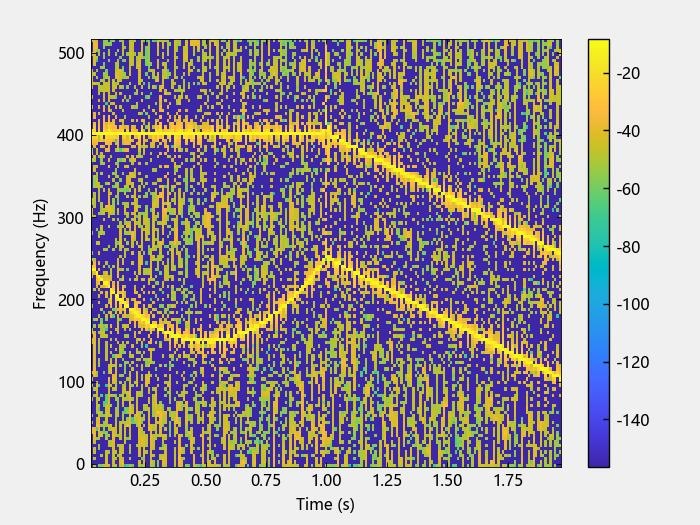
\includegraphics{hw5(8)-3.jpeg}
		\caption{Listing8结果图3}
		\label{fig8-3}
	\end{figure}
	\begin{figure}[htbp]
		\centering
		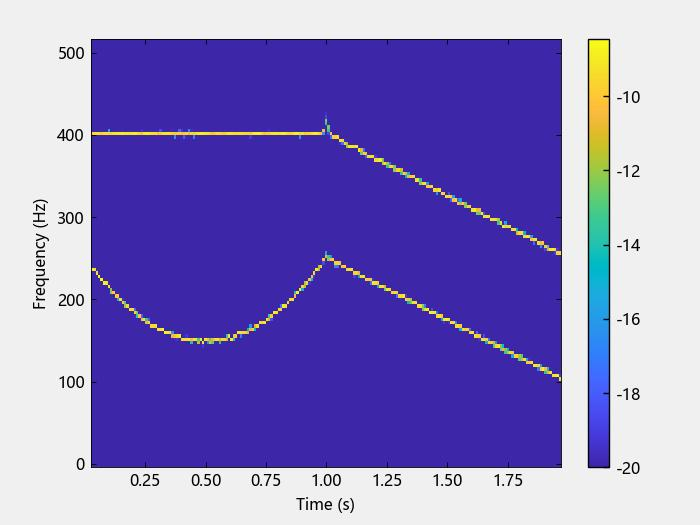
\includegraphics{hw5(8)-4.jpeg}
		\caption{Listing8结果图4}
		\label{fig8-4}
	\end{figure}
	\lstinputlisting[caption={三维频谱图可视化}, label={julia9}]{hw5(9).jl}
	\begin{figure}[htbp]
		\centering
		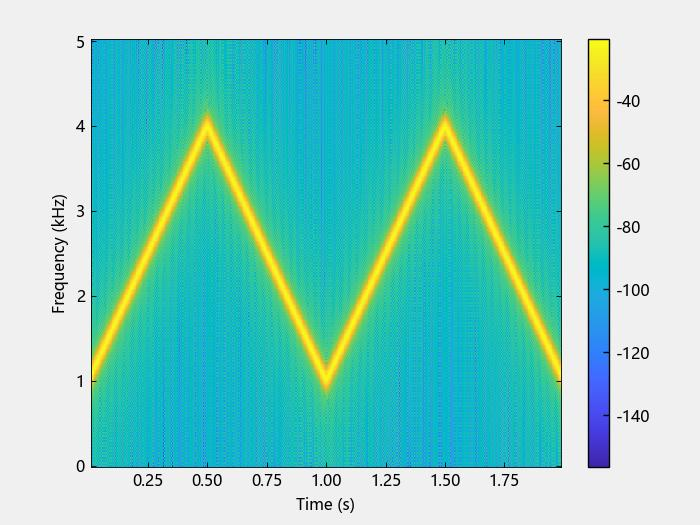
\includegraphics{hw5(9).jpeg}
		\caption{Listing9结果图}
		\label{fig9}
	\end{figure}
	
	\section*{xspectrogram}
	
	\begin{minted}{julia}
		s, = xspectrogram(x, y)
	\end{minted}
	
	返回 x 和 y 指定的信号的交叉频谱图。输入信号必须是元素数量相同的矢量。s 的每一列都包含 x 和 y 共同的短期、时间局部化频率内容的估计。
	
	\begin{minted}{julia}
		s, = xspectrogram(x, y, window)
	\end{minted}
	
	 使用 window 将 x 和 y 划分为多个分段并执行开窗操作。
	
	\begin{minted}{julia}
		s, = xspectrogram(x, y, window, noverlap)
	\end{minted}
	
	使用相邻线段之间重叠的 noverlap 样本。
	
	\begin{minted}{julia}
		s, = xspectrogram(x, y, window, noverlap, nfft)
	\end{minted}
	
	使用 nfft 采样点来计算离散傅立叶变换。
	
	\begin{minted}{julia}
		s, w, t = xspectrogram(___)
	\end{minted}
	
	返回归一化频率的矢量w和计算交叉频谱图的时刻的矢量 t。此语法可以包括以前语法中输入参数的任何组合。
	
	\begin{minted}{julia}
		s, f, t = xspectrogram(___, fs)
	\end{minted}
	
	返回频率向量 f,用采样率 fs 表示。fs 必须是 xsspectrogram 的第六个输入。要输入采样率并仍然使用前面可选参数的默认值,请将这些参数指定为空。
	
	\begin{minted}{julia}
		s, w, t = xspectrogram(x, y, window, noverlap, w)
	\end{minted}
	
	返回 w 中指定的归一化频率下的交叉频谱图。
	
	\begin{minted}{julia}
		s, f, t = xspectrogram(x, y, window, noverlap, f, fs)
	\end{minted}
	
	返回 f 中指定频率的交叉频谱图。
	
	\begin{minted}{julia}
		___, c = xspectrogram(___)
	\end{minted}
	
	还返回一个矩阵 c,该矩阵包含输入信号的时变复互谱的估计。交叉谱图 s 是 c 的大小。
	
	\begin{minted}{julia}
		___ = xspectrogram(___, freqrange)
	\end{minted}
	
	返回 freqrange 指定频率范围内的交叉谱图。freqrange 的有效选项为 "onesided"、"twosided" 和 "centered"。
	
	\begin{minted}{julia}
		___ = xspectrogram(___, Name, Value)
	\end{minted}
	
	使用名称-值对参数指定其他选项。选项包括最小阈值和输出时间维度。
	
	\begin{minted}{julia}
		___ = xspectrogram(___, spectrumtype)
	\end{minted}
	
	如果频谱类型指定为 "psd",则返回短期交叉功率谱密度估计值;如果频谱类型指定为 "power",则返回短期交叉功率谱估计值。
	
	\begin{minted}{julia}
		xspectrogram(___)
	\end{minted}
	
	在没有输出参数的情况下,在当前图形窗口中绘制交叉频谱图。
	
	\begin{minted}{julia}
		xspectrogram(___, freqloc)
	\end{minted}
	
	指定绘制频率的轴。将 freqloc 指定为 "xaxis" 或 "yaxis"。
	
	\lstinputlisting[caption={线性线性调频交叉频谱图}, label={julia10}]{hw5(10).jl}
	\begin{figure}[htbp]
		\centering
		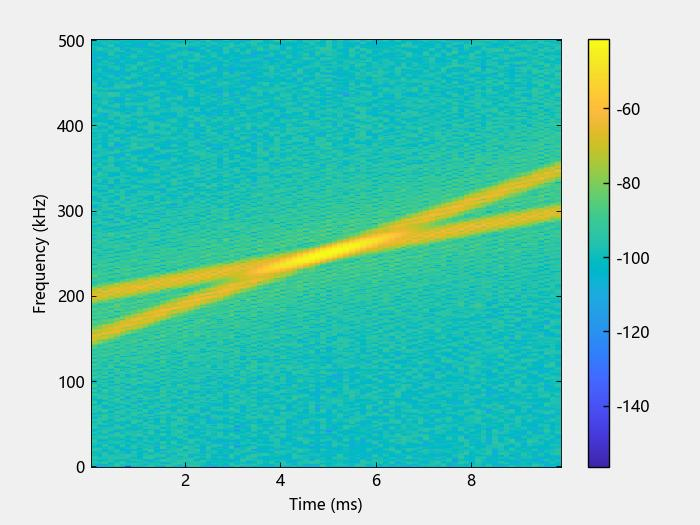
\includegraphics{hw5(10)-1.jpeg}
		\caption{Listing10结果图1}
		\label{fig10-1}
	\end{figure}
	\begin{figure}[htbp]
		\centering
		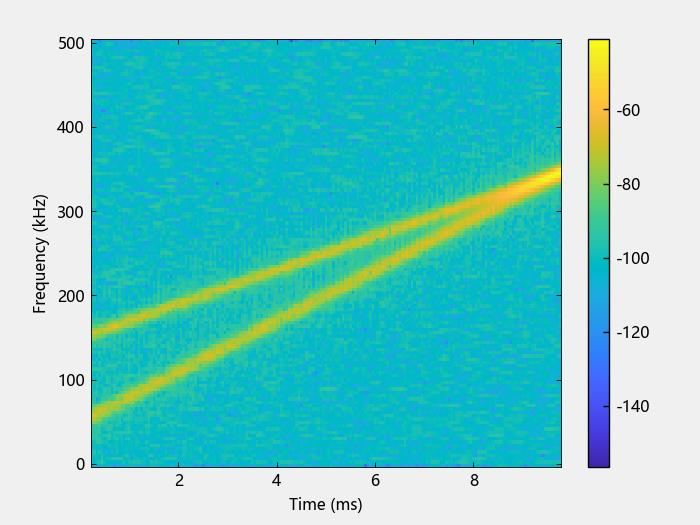
\includegraphics{hw5(10)-2.jpeg}
		\caption{Listing10结果图2}
		\label{fig10-2}
	\end{figure}
	\lstinputlisting[caption={两个二次线性调频之间的相移}, label={julia11}]{hw5(11).jl}
	\begin{figure}[htbp]
		\centering
		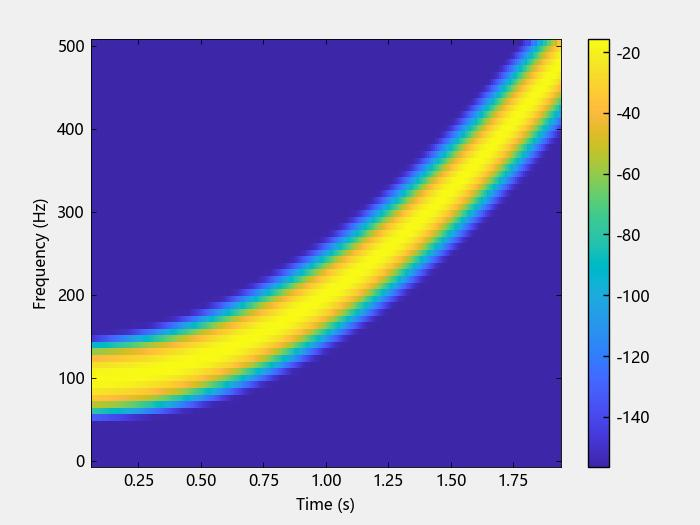
\includegraphics{hw5(11).jpeg}
		\caption{Listing11结果图}
		\label{fig11}
	\end{figure}
	\lstinputlisting[caption={复信号交叉谱图}, label={julia12}]{hw5(12).jl}
	\begin{figure}[htbp]
		\centering
		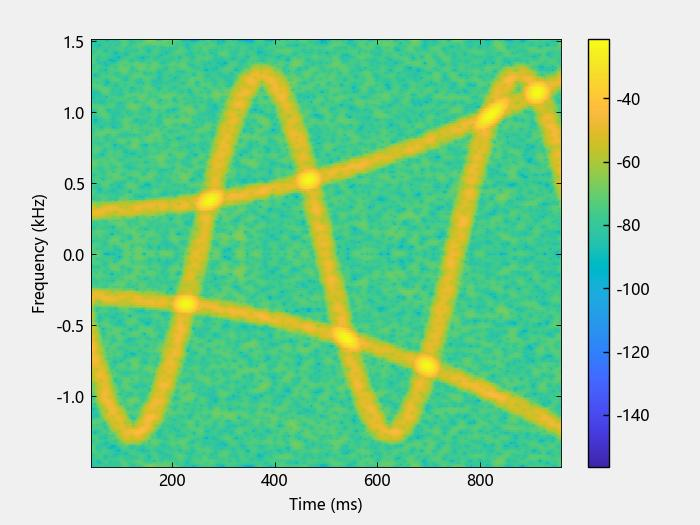
\includegraphics{hw5(12)-1.jpeg}
		\caption{Listing12结果图1}
		\label{fig12-1}
	\end{figure}
		\begin{figure}[htbp]
		\centering
		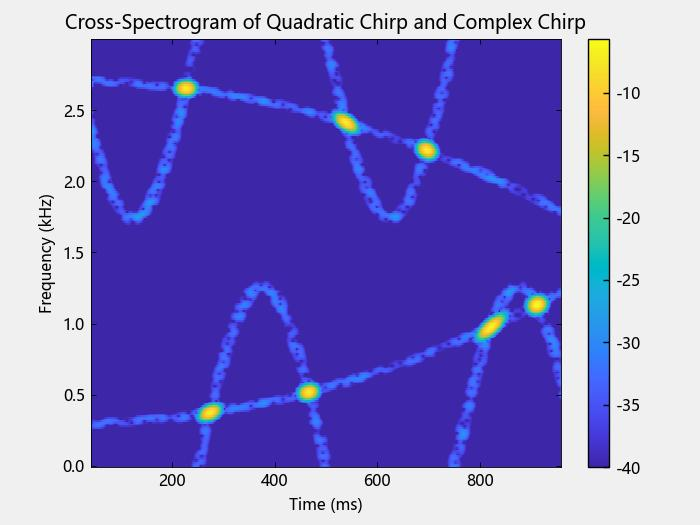
\includegraphics{hw5(12)-2.jpeg}
		\caption{Listing12结果图2}
		\label{fig12-2}
	\end{figure}
	\lstinputlisting[caption={两个序列的交叉谱图}, label={julia13}]{hw5(13).jl}
	\begin{figure}[htbp]
		\centering
		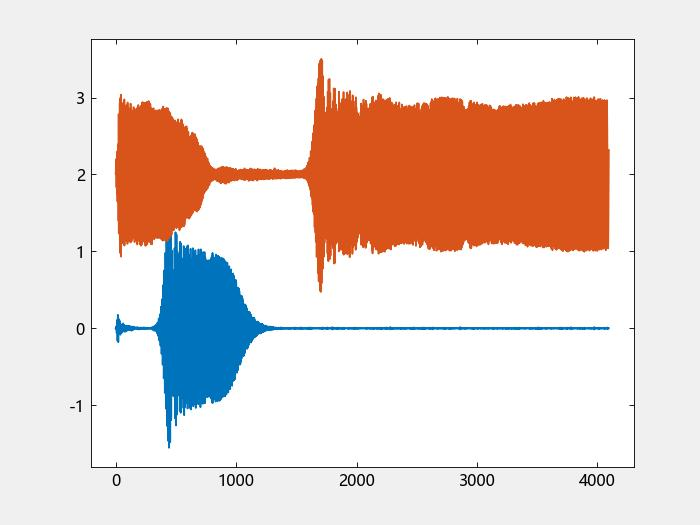
\includegraphics{hw5(13)-1.jpeg}
		\caption{Listing13结果图1}
		\label{fig13-1}
	\end{figure}
	\begin{figure}[htbp]
		\centering
		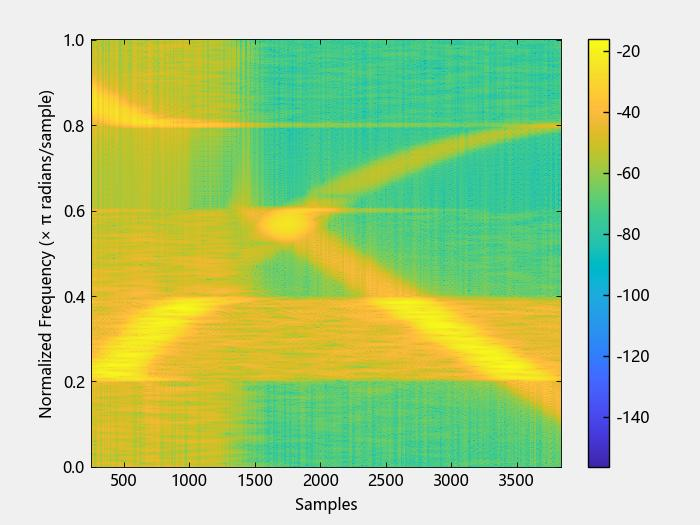
\includegraphics{hw5(13)-2.jpeg}
		\caption{Listing13结果图2}
		\label{fig13-2}
	\end{figure}
	\begin{figure}[htbp]
		\centering
		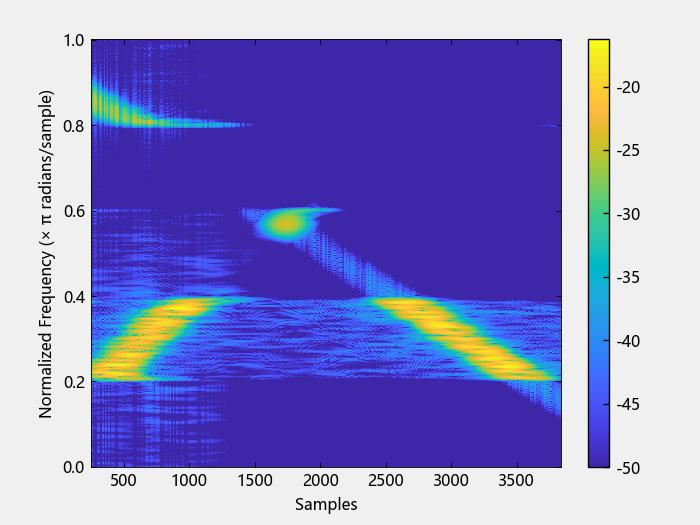
\includegraphics{hw5(13)-3.jpeg}
		\caption{Listing13结果图3}
		\label{fig13-3}
	\end{figure}
	
	\section*{stft}
	
	\begin{minted}{julia}
		s, = stft(x)
	\end{minted}
	
	返回 x 的短时傅立叶变换 (STFT)。
	
	\begin{minted}{julia}
		s, = stft(x,fs)
	\end{minted}
	
	使用采样率 fs 返回 X 的 STFT。
	
	\begin{minted}{julia}
		s, = stft(___;Name = Value)
	\end{minted}
	
	使用名称=值参数对指定其他选项。选项包括 FFT 窗口长度和重叠样本数。这些参数可以添加到任何先前的输入语法中。
	
	\begin{minted}{julia}
		s,f, = stft(___)
	\end{minted}
	
	返回评估 STFT 的信号频率。
	
	\begin{minted}{julia}
		s,f,t = stft(___)
	\end{minted}
	
	返回评估 STFT 的信号时间。
	
	\lstinputlisting[caption={短时傅里叶变换}, label={julia14}]{hw5(14).jl}
	\begin{figure}[htbp]
		\centering
		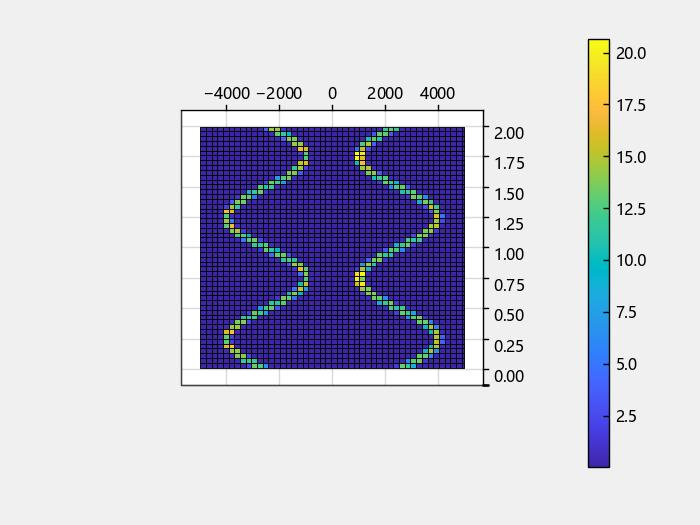
\includegraphics{hw5(14).jpeg}
		\caption{Listing14结果图}
		\label{fig14}
	\end{figure}
	\lstinputlisting[caption={扫频余弦信号STFT}, label={julia15}]{hw5(15).jl}
	\begin{figure}[htbp]
		\centering
		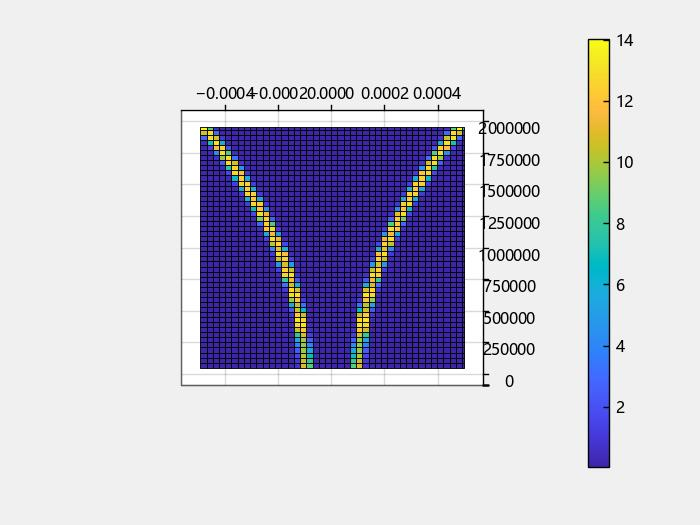
\includegraphics{hw5(15).jpeg}
		\caption{Listing15结果图}
		\label{fig15}
	\end{figure}
	\lstinputlisting[caption={STFT频率范围}, label={julia16}]{hw5(16).jl}
	\begin{figure}[htbp]
		\centering
		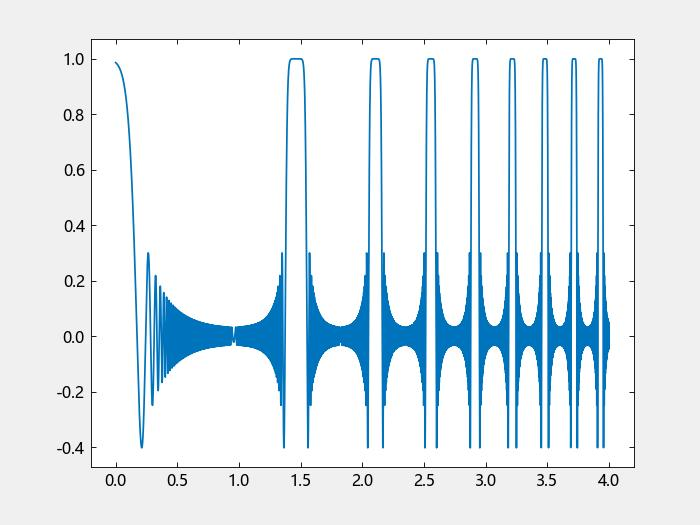
\includegraphics{hw5(16)-1.jpeg}
		\caption{Listing16结果图1}
		\label{fig16-1}
	\end{figure}
	\begin{figure}[htbp]
		\centering
		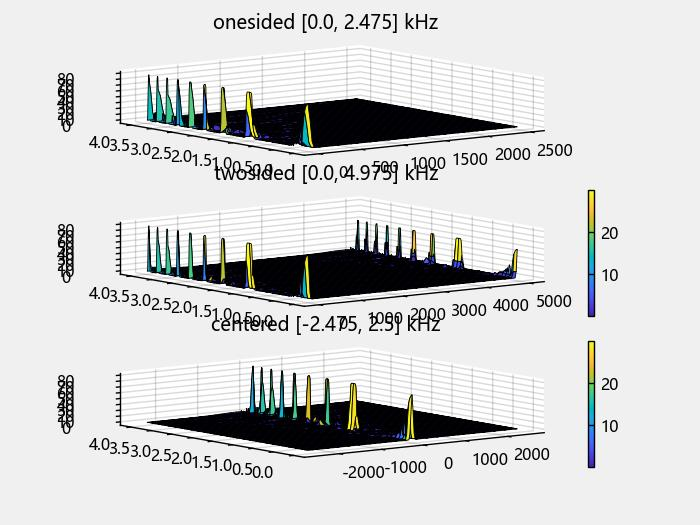
\includegraphics{hw5(16)-2.jpeg}
		\caption{Listing16结果图2}
		\label{fig16-2}
	\end{figure}
	\begin{figure}[htbp]
		\centering
		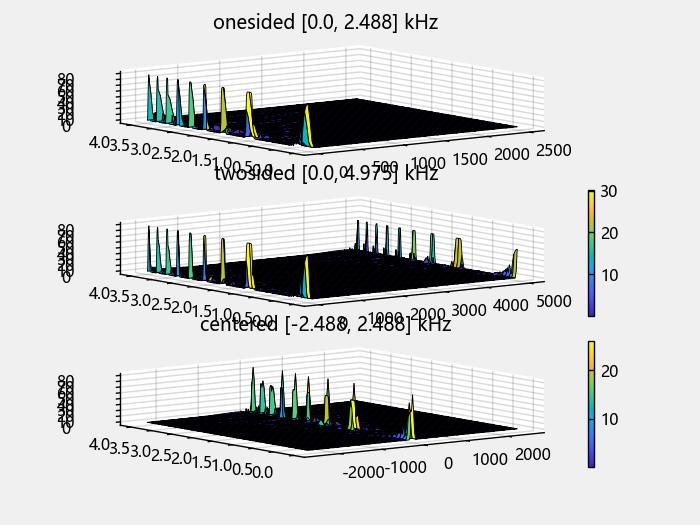
\includegraphics{hw5(16)-3.jpeg}
		\caption{Listing16结果图3}
		\label{fig16-3}
	\end{figure}
	
	\section*{iscola}
	
	\begin{minted}{julia}
		b = iscola(window,noverlap)
	\end{minted}
	
	检查指定的窗口和重叠是否满足恒定重叠相加 (COLA) 约束,以确保逆短时傅立叶变换对未修改的光谱产生完美的重建。
	
	\begin{minted}{julia}
		b = iscola(window,noverlap,method)
	\end{minted}
	
	指定要使用的反演方法。
	
	\begin{minted}{julia}
		b,m= iscola(___)
	\end{minted}
	
	还返回 COLA 总和的中位数。 您可以将这些输出参数与任何先前的输入语法一起使用。
	
	\begin{minted}{julia}
		b,m,maxDeviation = iscola(___)
	\end{minted}
	
	返回与中位数 m 的最大偏差。
	
	\lstinputlisting[caption={COLA合规性}, label={julia17}]{hw5(17).jl}
\end{document}
